\documentclass[11pt,a4paper]{article}
\usepackage[utf8x]{inputenc}
\usepackage[T1]{fontenc}
%\usepackage{gentium}
\usepackage{mathptmx} % Use Times Font
\usepackage{mathtools}
\usepackage{float}
\usepackage{graphicx} % Required for including pictures
\usepackage{hyperref} % Format links for pdf
\usepackage[british]{babel} % Multilingual bibliographies
\usepackage{natbib}
\setlength{\bibsep}{0.0pt}
\usepackage{multicol}
\usepackage{booktabs}
\frenchspacing % No double spacing between sentences
\usepackage[margin=1in]{geometry}
\usepackage{enumitem}
\setitemize{noitemsep,topsep=0pt,parsep=0pt,partopsep=0pt}

\usepackage[all]{nowidow} % Tries to remove widows
\usepackage[protrusion=true,expansion=true]{microtype} % Improves typography, load after fontpackage is selected

\usepackage{lipsum} % Used for inserting dummy 'Lorem ipsum' text into the template

\title{FDS Final Project\\Variability of UK Higher Education grades}
\author{Mrinmoy Sonowal and Kuan Lon Vu}
%\usepackage{natbib}

\begin{document}

\maketitle

%% INSTRUCTIONS:
%%
%% 1. Please rename this file fds-project-option-1.tex,
%% fds-project-option-2.tex, or fds-project-option-3.tex, depending on
%% which project option you are doing. When you submit, please submit
%% the PDF file with the corresponding name.
%% 
%% 2. You can edit either using:
%%
%%    a. Overleaf professional, a collaborative LaTeX editor. See
%%       https://www.overleaf.com/edu/edinburgh for documentation. Create an
%%       empty document, and copy the files in this directory to it.
%%
%%    b. A LaTeX editor on your PC - you can commit changes to this
%%       repository to collaborate.
%% 
%% 3. Please keep the section and paragraph headings as they are.
%%
%% 4. The word limit for the Overview section is mandatory. For the
%% other sections word limits are suggested.
%%
%% 5. The page limits must be strictly adhered to, and depend on if
%% you are working individually, in pairs or in threes:
%%
%%   - Individual: 6 pages 
%%   - Pairs: 8 pages 
%%   - Threes: 10 pages 
%%

\section{Overview}
% 250 words maximum
For several years, grade inflation in higher education degree classification has been a topic of great interest for many stakeholders in the public, government, education sector and industry. It is worried that a continuous increase in the proportion of the top degrees would be unfair for hardworking students from previous years \cite{end_inflation}. In this report, we investigated the supposed increase in proportion of 'First class' degrees per year and the odds of receiving First class within different demographic groups. 
We found that the increase in proportion of ‘First class’ degrees in 2019/20 is statistically significant. There was no statistically significant increase from 2014/15 to 2016/17 and from 2017/18 to 2018/19. The statistical significance was tested using the 95\% confidence interval (CI). We studied the odds being awarded a ‘First class’ degree by the University of Edinburgh. We found that there is a greater chance of receiving a ‘First class’ degree from the University of Edinburgh in 2019/20 compare to 2018/2019. We found that there is a disparity between different demographic groups at attaining a ‘First class’ degree. We measured the odds ratios of being awarded a First class for each demographic group, and tested their statistical significance using 95\% CIs. We acquired the data from HESA and performed preliminary analysis to find gradual increases in ‘First class’ attainment by plotting stacked barchart and boxplots. We later calculated the odds ratios and 95\% CIs for mean proportion of ‘First class’ per year, and plotted these on graphs.


\section{Introduction}
% Suggested 400 words

\paragraph{Context and motivation}

This study is an observational longitudinal retrospective cohort study. This is because we have used existing datasets collected from the universities over several years without any interventions. Those datasets are used to detect changes in the number of each degree classification over the sample years and examine whether the odds vary across those years for different demographic groups.
Degree classifications in the UK are as follows: First class honours, Upper second class honours, Lower second class honours, Third class honours, and unclassified degrees.
As university students, we are interested in understanding the issue of grade inflation as well as understanding our own odds in getting a first, given multiple demographic data points. Degree inflation, caused due to grade inflation, is defined as the decrease in value as a result of more number of students achieving a 'good' degree classification. This can be due to a wide range of factors, including, making exams easier, inflating grades to maintain university reputation or just improvements in learning outcomes \cite{Bachan_2015}.
The topic of degree classifications has also been frequently been reported in media and has been a cause of concern for numerous students as jobs get more competitive and the value of the degree diminishes. This study is aimed at finding out if degree inflation is a growing problem by analysing degree classification and achievement data from 2014/15 to 2019/20. \cite{Weale_2020}\cite{Coughlan_2019}.
\paragraph{Previous work}
The 2020 Office for Students (OfS) report investigated and analysed the pattern in the change in the proportion of the First and Upper Second class degrees awarded between 2010/11 to 2018/19 \cite{OfS_2020}. There is also a related news article from the Guardian reporting on the OfS report \cite{Weale_2020}. Moreover, research paper from 2015 discussed that the modularisation of degree programmes and the change in assessment methods may have contributed to the increase in First and Upper second class honours degrees \cite{Bachan_2015}. Bachan (2015) also further discussed other possible causes of such increase such as overall increase in student motivation and student ability, and the use of better teaching methods.

The Higher Education Statistics Agency (HESA) report in 2003 found that females gain more first degrees than males when combining first class and upper second class degrees together \cite{HESA_2003}.

\paragraph{Objectives}

In this report we would like to explore the following:
\begin{enumerate}
    %\item The difference in proportion of each degree classification from the different higher education (HE) providers from 2014/15 to 2019/20. This is because by identifying any increase or decrease in the proportion of degree classifications, it can help detect grade inflation in those years.
    \item We are going to investigate if degree inflation in UK universities is still a recurring phenomenon. We would use the data provided by HESA from the years 2014/15 to 2019/20 and study the extent of degree inflation in these years.
    \item Next, we study the degree classifications awarded by the University of Edinburgh from the academic years 2014/15 to 2019/20. We analyse if degree inflation is prevalent in this university as well as explore the odds of achieving a first class as compared to other universities.
    \item The HESA report in 2003 says that certain demographic groups have greater odds of receiving a First class honour degree \cite{HESA_2003}. Therefore, we would like to investigate if this is continuing, i.e., the odds of being awarded First class honour is higher in certain groups than in others, in the years 2014/15 to 2019/20.
\end{enumerate}
 %We chose to investigate the proportion rather than the actual number of degree classification from the HE provider because there are varying number of total number of first degree qualifications awarded by each provider every year. 
% To investigate the HE providers with highest and lowest proportions of each degree classification across per year, to identify any consistency or patterns in those providers. 



\section{Data}
% Suggested 300 words

\paragraph{Data provenance} 
To investigate the objectives, we have used 2 datasets in total. The data from both datasets were collected by the HESA from higher education (HE) providers in the UK. HESA is the official government agency for collecting data about UK higher education. They collect a range of data from HE providers annually which complies to GDPR, and subsequently enabling other government departments and HE funding bodies to base their work on the data provided by HESA \cite{Imperial_HESA}. Therefore, data from HESA is a reliable source to base this investigation on. The website cited below contained several csv files that were downloaded and cleaned for the purpose of this project. As this data had an open data licence (CC-BY-4.0 \cite{CreativeCommons}), we were sure that the data can be used liberally as long as the providers are cited. \cite{HESA_Intro}
\paragraph{Data description} 
\begin{enumerate}
  \item The first dataset \textit{(providers)} includes the level of qualification data, such as foundation degree, master taught etc. and first degree classification data of 297 HE providers from 2014/15 to 2019/20. This dataset is chosen as the first degree classification data includes data on the different type of degree classifications and degree types by higher education centres in the United Kingdom, which is relevant to the objectives we are exploring. \cite{UKPRN_Data_1}. (Number of records: 114408) 
  \begin{multicols}{2}
  \begin{itemize}
      \item \textbf{UKPRN} - UK Provider Reference Number \cite{UKPRN}
      \item \textbf{HE provider} - Name of higher education provider
      \item \textbf{Country of HE provider} - England/Wales/Scotland/NI
      \item \textbf{Region of HE provider} - Regions of the UK - East Midlands, North East etc.
      \item \textbf{Academic Year} - From 2014/15 to 2019/20
      \item \textbf{Qualification/Classification marker}
      \begin{itemize}
            \item \textbf{Level of qualification} - First degree, Postgraduate degree, Foundation, etc.
            \item \textbf{First degree classification} - First class, second class, etc.
      \end{itemize}
      \item \textbf{Level of qualification/Degree classification}
      \item \textbf{Number} - Number of degrees
  \end{itemize}
  \end{multicols}
  
  \item The second dataset \textit{(factors)} contains the data for domiciled students from 2014/15 to 2019/20. The following are the list of data point columns it contains. (Number of records: 8725)
  \begin{multicols}{2}
  \begin{itemize}
      \item \textbf{Category Marker} - sex, ethnicity, disability status etc. 
      \item \textbf{Category} - Name of higher education provider
      \item \textbf{Mode of study} - Full-time or Part-time
      \item \textbf{Country of HE provider} - \\England/Wales/Scotland/Northern Ireland
      \item \textbf{Academic Year} - From 2014/15 to 2019/20
      \item \textbf{Classification of first degree} -
      \begin{itemize}
          \item First class, upper second class, lower second class, third class and unclassified
      \end{itemize}
      \item \textbf{Number} - Number of degrees
  \end{itemize}
  \end{multicols}

  This data separates the degree class achieved by students by their demographic data and country of origin, as well as their mode of study. A row of the data would give us the number of degrees received by a demographic group, for a particular year, mode of study and country. This dataset is chosen as it provides the data to investigate the odds of First class with the different demographic data.
  Note that this degree dataset has fewer number of degrees  than the first dataset.
\end{enumerate}


\begin{figure}[t]
  \centering
  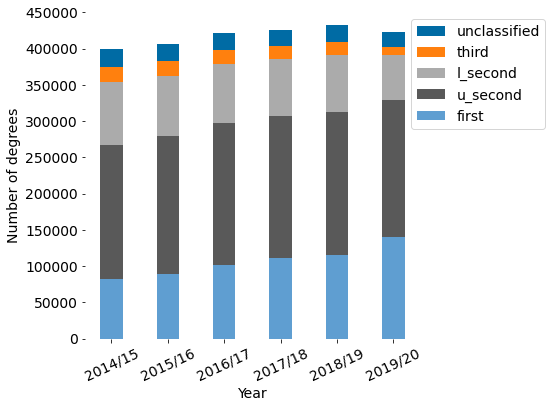
\includegraphics[scale=0.6]{figures/Stacked_Bar_Chart.png}
  \caption{The distribution of the degree classifications within the total given degrees per year}
  \label{stacked-barchart}
\end{figure}
\paragraph{Data processing} 
% \subparagraph{}
\begin{itemize}
    \item Cleaning \textit{providers} dataset - 
    We split the csv file as it was very cluttered, for instance, the sum of data  and the definition of the data were included in the same file. The different classifications dataset allowed us to see how the number of degrees achieved changed over the years. We then removed all the rows that contained fields such as, 'All' and 'Total' as they were redundant. We only included individual university data for different first degree classifications. We also removed all the NaN values as they couldn't be used. Next, we split our classification pandas' dataframe by each first degree classification, ie., First, Upper Second, Lower Second, Third and Unclassified.

    \item Cleaning \textit{factors} dataset -
    This dataset contained all the demographic groups as well as the description in one csv file. First the description was moved to another file. Using pandas, we then split the data set into multiple csv files separated by the category field, i.e., datasets for sex, ethnicity, disability status, etc. were created. Next using pandas we acquired the data for each group and created a dataframe, and from each dataframe we considered the data-points that achieved a first degree classification. Age Unknown field was removed from this data set, as it didn't have any number of degrees.
\end{itemize}
\section{Exploration and  analysis}
% Suggested 500 words for individual report; proportionately longer
% for group projects).
% 't' means "try to position at the top of the page"

Figure~\ref{stacked-barchart} shows that there is a general increase with the number of First class degrees as the years go on, whilst the number of Upper Second class degrees has remained fairly constant over the sample years. On the complementary, the number of Third class and Lower Second class degrees have been decreasing over the sample years. This increase in First class and decrease in lower honours degree might be contributed by the wider availability of information, allowing easier and quicker access to resources which enables students to gain better grades in their assessments. Moreover, notice the greater increase of First class degrees awarded in 2019/20 compare to rest of the years, and is statistically significant when comparing to 2018/19. This could be influenced by the sudden change of methods of assessment caused by the COVID-19 pandemic, forcing many honours examinations to be taken online instead. To address the sudden disruption of studies, many universities also had the non-detriment policy in-place which ensured students would be awarded a final grade that is no less than their previous in-year assessment \cite{Guardian_2020_grade_inflation}.

\begin{figure}[t]
    \centering
    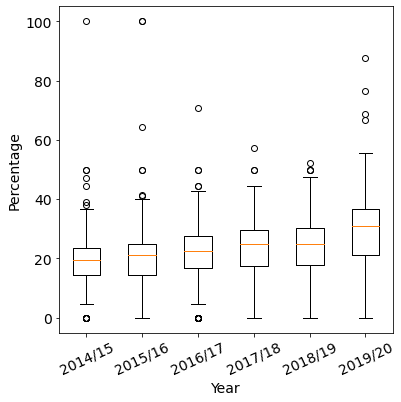
\includegraphics[scale=0.6]{figures/First_Prop_BoxPlt.png}
    \caption{Visual summary of distribution of the proportion of First class degree classification by year}
    \label{first-class-prop-boxplot}
\end{figure}

% \begin{figure}[h]
%     \centering
%     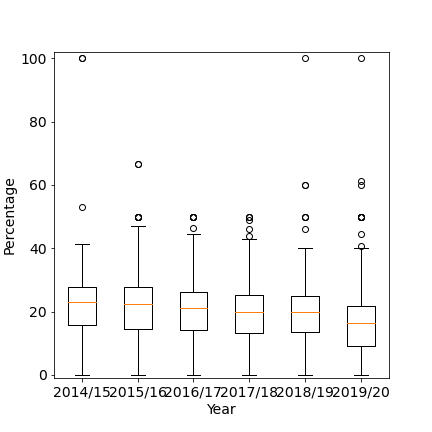
\includegraphics[scale=0.6]{figures/Third_Prop_BoxPlt.png}
%     \caption{Boxplot showing the proportion of Third class degree classification by year}
%     \label{third-class-prop-boxplot}
% \end{figure}

We also looked at the proportion of First class degrees (Figure~\ref{first-class-prop-boxplot}) from the higher education (HE) providers from 2014/15 to 2019/20. This is because by identifying any increase or decrease in the proportion of those degree classifications, it can help detect grade inflation in those years. We chose to investigate the proportion rather than the actual number of degree classification from the HE provider because there are varying number of providers each year. In Figure~\ref{first-class-prop-boxplot} shows that the distributions are near normal and symmetric distributions.

% Figure~\ref{third-class-prop-boxplot} shows a similar finding except for year 2019/20, which its distribution is slightly negative-skewed and asymmetric.


To measure the uncertainty in the calculated proportions of First class degrees across 2014/15 to 2019/2020, we calculated the 95\% confidence intervals. 

Formula for the 95\% confidence interval for the mean proportion of First class degree classification:
\setlength{\belowdisplayskip}{4pt} \setlength{\belowdisplayshortskip}{4pt}
\setlength{\abovedisplayskip}{4pt} \setlength{\abovedisplayshortskip}{4pt}
\begin{equation}
    CI = \exp{\left[ \overline{x} \pm \overbrace{1.96}^\text{z-score}\times\overbrace{\frac{\sigma}{\sqrt{n}}}^\text{SE of mean}\right]}
\end{equation}
Where:\\
$\overline{x}$ = the mean proportion of First class degrees in that year\\ 
$\sigma$ = the standard deviation \\
$n$ = the number of universities concerned\\

As shown in Figure~\ref{first-class-prop-CI-plot}, we for example, can be 95\% confident that the proportion of the first class degrees in 2014/15 is 18.41 and 21.32, and in 2019/20 is between 26.51 and 30.26 (all values quoted to 2 d.p.). Figure~\ref{first-class-prop-CI-plot} also shows that it the proportion of degrees with First class honours in 2019/20 are statistically significant as there is no overlap when comparing 2019/20 to the rest of the years. The overlaps from 2014/15 to 2016/17 and 2017/18 to 2018/19 indicate that whilst the ranges of proportion of first class degrees have shifted to the right (increased) over those years, the true proportion of the population may not have increased, hence they are not statistically significant. Moreover, it should be noted that the increase in proportion of first class degrees in 2017/18 from 2014/15 is statistically significant.

Figure~\ref{CI_OR_UOE} shows that for years 2015/16, 2016/17 and 2019/20, there is a greater chance of being awarded a First class degree by the University of Edinburgh. The greater increase in the odds in year 2019/20 could be due to examinations with adapted format to allow remote assessment, and the University's participation in the non-detriment policy to support students \cite{UOE_Covid_assessment_policy}. Therefore the average grades of the final year students could only be equal to or higher than the grades from the assessments already taken that year. Moreover, this increase in 2019/20 matches the increase in total number of First class degrees in 2019/20 shown in Figure~\ref{stacked-barchart}.

\begin{figure}[t]
    \centering
    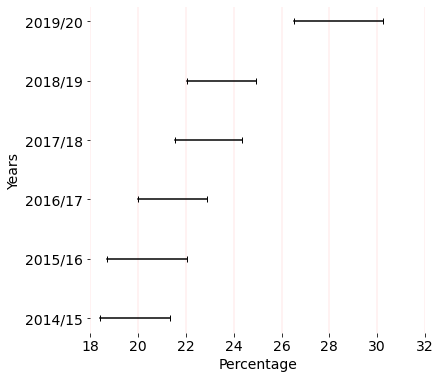
\includegraphics[scale=0.6]{figures/CI_First_Prop_plot.png}
    \caption{Confidence interval of the mean proportion of First class degrees per year}
    \label{first-class-prop-CI-plot}
\end{figure}

\begin{figure}[t]
    \centering
    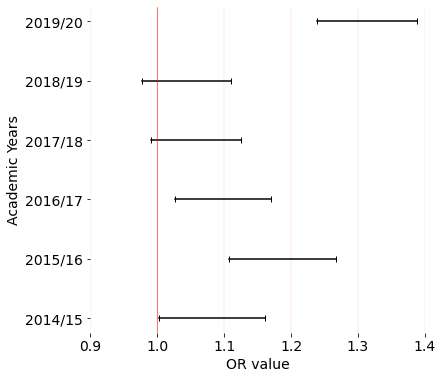
\includegraphics[scale=0.6]{figures/CI_OR_UOE.png}
    \caption{Confidence intervals of the odds ratio for First class degrees awarded in the University of Edinburgh by year.}
    \label{CI_OR_UOE}
\end{figure}

\subsection{Odds ratios of receiving First class degrees for different demographic groups}
Odds ratios (OR) are used to compare the odds of receiving First class degrees, given exposure to each demographic group in Table~\ref{tab:demographic_OR_CI}. This is because when the OR of a particular demographic data is greater than 1, it means that demographic group is associated with greater chance of First class degrees.

To find out whether the odds ratios of being awarded First class across 2014/15 to 2019/20 for each demographic group are statistically significant or rather due to chance, we calculated the 95\% confidence intervals for those odds ratios as shown in Table~\ref{tab:demographic_OR_CI}. This is because if the 95\% CI of an OR includes 1, then that OR is not statistically significant.
\newline
\setlength{\belowdisplayskip}{4pt} \setlength{\belowdisplayshortskip}{4pt}
\setlength{\abovedisplayskip}{4pt} \setlength{\abovedisplayshortskip}{4pt}
Formula for calculating the odds ratio for each demographic category:
\begin{equation}
    \label{fds-project-template:demographic_odds_ratio_eq}
    OR =\frac{a/c}{b/d} = \frac{ad}{bc}
\end{equation}
Formula for 95\% Confidence Interval for the odds ratio \cite{NCBI_Odds_ratio}:
\setlength{\belowdisplayskip}{4pt} \setlength{\belowdisplayshortskip}{4pt}
\setlength{\abovedisplayskip}{4pt} \setlength{\abovedisplayshortskip}{4pt}
\begin{equation}
    \label{fds-project-template:demographic_ci_odds_ratio_eq}
    CI = \exp{\left[\ln{(OR)}\pm\overbrace{1.96}^\text{z-score}\times\underbrace{\sqrt{ \frac{1}{a} + \frac{1}{b}+ \frac{1}{c} + \frac{1}{d}}}_\text{SE of ln(OR)}\right]}
\end{equation}
Where:\\
$a$ = Number for firsts for that group \quad $b$ = Number of all other degrees for that group\\
$c$ = Number of firsts for other groups \quad $d$ = Number of other degrees for other groups\\

Therefore, the following is the breakdown of the odds ratio for each demographic groups (Table~\ref{tab:demographic_OR_CI}).
\begin{itemize}
\begin{multicols}{2}
    \item For the category of sex:
    \begin{itemize}
        \item $OR > 1$: Female, Other
        \item $OR < 1$: Male
        \item Statistically Insignificant: Not known
    \end{itemize} 
    \item For the category of ethnicity:
    \begin{itemize}
        \item $OR > 1$: White
        \item $OR < 1$: Black, Asian, Mixed, Other, Not known
    \end{itemize}
    \end{multicols}
    \item For the category of religious belief:
    \begin{itemize}
        \item $OR > 1$: No religion, Jewish
        \item $OR < 1$: Buddhist, Christian, Hindu, Muslim, Sikh
        \item Statistically Insignificant: Spiritual, Any other religion or belief, Not known
    \end{itemize}
    \begin{multicols}{2}
    \item For the category of age group:
    \begin{itemize}
        \item $OR > 1$: 21-24 years
        \item $OR < 1$: 20 and under, 25-29 years
        \item Statistically Insignificant: 30 years  \\and over\\
    \end{itemize}
    \item For the category of disability status
    \begin{itemize}
        \item $OR > 1$: No known disability 
        \item $OR < 1$: Known disability
    \end{itemize}
    \end{multicols}
\end{itemize}
The odds are 1.6630 (1.6496-1.6765) times higher that a white student would receive a First class degree compared to a non-white student. White is the only demographic group on the category of ethnicity that has a increased odds of receiving a First class degree. Moreover, the odds ratios for Black is 0.4202 (0.4133-0.4272) and Asian is 0.7293 (0.7213-0.7374) with Black and White having the largest difference in odds ratio. This reflects the degree attainment gap for the minority ethnic groups in the UK HE student population which universities are trying to tackle \cite{BAME_attainment_gap}.
As the standard error (SE) of the log OR increases, the greater the range shown in the CI. Notice for the category of sex, the SE of the log OR for 'Not known' (OR=0.9178, 0.5533-1.5224) is 0.2582 - greater than the SEs of ln(OR) for the other 3 groups. Therefore 'Not known' has the largest range for its 95\% CI of OR. This is because the smaller the number of data (i.e. number of Sikhs receiving a First class) we have on a particular group, the larger their SE of ln(OR), resulting in a increased CI range. This is also true for '20 and under' as there are few UK-domiciled students who graduate age 20 or under. 
% female OR = 1.0425 (95\% CI 1.0357-1.0493)
% male OR = 0.9586 (95\% CI 0.9524-0.9649)

\begin{table}[t]
    \caption{Confidence Interval Table for First class degree odd ratios for each demographic}
    \label{tab:demographic_OR_CI}
\begin{center}
\begin{tabular}{lrrrr}
\toprule
                    Demographic group &  Odds ratio &  Lower 95\% CI &  Upper 95\% CI &  Standard error of ln(OR)\\
\midrule
                      Female &      1.0425 &              1.0357 &              1.0493 &          0.0033 \\
                        Male &      0.9586 &              0.9524 &              0.9649 &          0.0033 \\
                       Other &      1.4413 &              1.2472 &              1.6655 &          0.0738 \\
                   Not known &      0.9178 &              0.5533 &              1.5224 &          0.2582 \\
\midrule                   
                       White &      1.6630 &              1.6496 &              1.6765 &          0.0041 \\
                       Black &      0.4202 &              0.4133 &              0.4272 &          0.0085 \\
                       Asian &      0.7293 &              0.7213 &              0.7374 &          0.0056 \\
                       Mixed &      0.9100 &              0.8946 &              0.9257 &          0.0087 \\
                       Other &      0.7201 &              0.6986 &              0.7423 &          0.0155 \\
                   Not known &      0.5569 &              0.5407 &              0.5736 &          0.0150 \\
\midrule                   
                 No religion &      1.2595 &              1.2463 &              1.2728 &          0.0054 \\
                    Buddhist &      0.8287 &              0.7616 &              0.9018 &          0.0431 \\
                   Christian &      0.8869 &              0.8767 &              0.8972 &          0.0059 \\
                       Hindu &      0.8410 &              0.8065 &              0.8770 &          0.0214 \\
                      Jewish &      1.2216 &              1.1325 &              1.3177 &          0.0386 \\
                      Muslim &      0.6440 &              0.6305 &              0.6578 &          0.0108 \\
                        Sikh &      0.8272 &              0.7836 &              0.8733 &          0.0276 \\
                   Spiritual &      0.9988 &              0.9506 &              1.0495 &          0.0252 \\
Any other religion or belief &      1.0272 &              0.9814 &              1.0751 &          0.0232 \\
                   Not known &      1.0161 &              0.9966 &              1.0359 &          0.0099 \\
\midrule                   
                20 and under &      0.8553 &              0.8385 &              0.8725 &          0.0101 \\
                 21-24 years &      1.0916 &              1.0826 &              1.1007 &          0.0042 \\
                 25-29 years &      0.8904 &              0.8796 &              0.9013 &          0.0062 \\
           30 years and over &      0.9885 &              0.9770 &              1.0001 &          0.0059 \\
\midrule           
            Known disability &      0.8993 &              0.8911 &              0.9075 &          0.0046 \\
         No known disability &      1.1119 &              1.1018 &              1.1221 &          0.0046 \\
\bottomrule
\end{tabular}
\newline
\end{center}
\end{table}

% \begin{figure}[H]
%     \centering
%     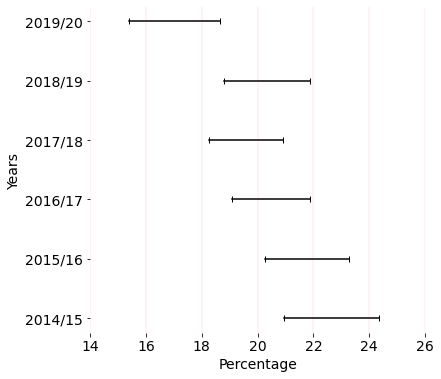
\includegraphics[scale=0.8]{figures/CI_Lower_Second_Prop_plot.png}
%     \caption{Confidence interval of the proportion of Lower Second class degrees per year}
%     \label{lower-second-class-prop-CI-plot}
% \end{figure}

% \begin{figure}[H]
%     \centering
%     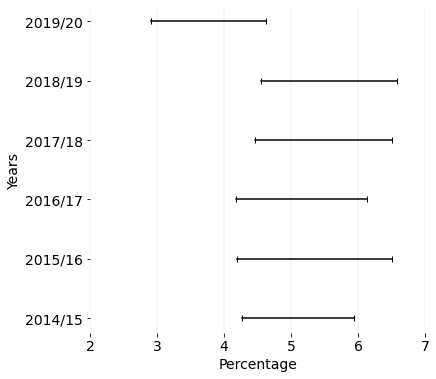
\includegraphics[scale=0.8]{figures/CI_Third_Prop_plot.png}
%     \caption{Confidence interval of the proportion of Third class degrees per year}
%     \label{third-class-prop-CI-plot}
% \end{figure}

% \begin{figure}[H]
%     \centering
%     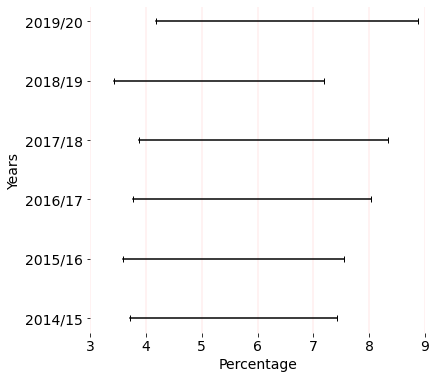
\includegraphics[scale=0.8]{figures/CI_Unclassified_Prop_plot.png}
%     \caption{Confidence interval of the proportion of Unclassified class degrees per year}
%     \label{unclassified-class-prop-CI-plot}
% \end{figure}

% 'b' means "try to position at the bottom of the page"
% \begin{table}[b]
%   \caption{Excerpt from Scottish Index of Multiple Deprivation, 2016 edition.
%     \url{https://simd.scot}. You may put more information in the caption.}
%   \label{tab:example1}
% \begin{tabular}{lrrrrrrr}
% \hline\hline
% \textbf{Location}&\textbf{Employ-}&\textbf{Illness}&\textbf{Attain-}&\textbf{Drive}  &\textbf{Drive}    &\textbf{Crime}&\dots\\
%                  &\textbf{ment}   &                &\textbf{ment}   &\textbf{Primary}&\textbf{Secondary}&              &\\
% \hline
% \textbf{Macduff}&$10$&$ 95$&$5.3$&$1.5$&$6.6$&$249$&\dots\tabularnewline
% \textbf{Kemnay}&$ 3$&$ 40$&$5.3$&$2.4$&$2.4$&$168$&\dots\tabularnewline
% \textbf{Hilton}&$ 0$&$ 10$&$6.3$&$2.2$&$3.0$&$144$&\dots\tabularnewline
% \textbf{Ruchill}&$ 8$&$130$&$4.9$&$1.7$&$5.6$&$318$&\dots\tabularnewline
% \textbf{Belmont}&$ 2$&$ 50$&$6.1$&$3.1$&$3.2$&$129$&\dots\tabularnewline
% \dots&\dots&\dots&\dots&\dots&\dots&\dots&\dots\tabularnewline
% \hline
% \end{tabular}
% \end{table}


% A data science analysis of the paper, including: 
% \begin{itemize}
% \item Visualisations (for example
%   Figure~\ref{stacked-barchart}) and tables (for
%   example Table~\ref{tab:example1}). Please make sure that all figures
%   and tables are referred to in the text, as demonstrated in this
%   bullet point.
% \item Interpretation of the results 
% \item Description of how you have applied one ore more of the
%   statistical and ML methods learned in the FDS to the data
% \item Interpretation of the findings 
% \end{itemize}

% You can use equations like this:
% \begin{equation}
%   \label{fds-project-template:eq:1}
%   \overline{x} = \sum_{i=1}^n x_i
% \end{equation}
% or maths inline: $E=mc^2$. However, you do not need to reexplain techniques that you have learned in the course -- assume the reader understands linear regression, logicstic regression K-nerest neighbours etc.  Remember to explain any symbols use, e.g.~``$n$ is the number of data points and $x_i$ is the value of the $i$th data point.''.

\section{Discussion and conclusions}
% Suggested 400 words.

\paragraph{Summary of findings}
\begin{enumerate}
    \item We found that from the sample years of 2014/15 to 2019/20, the sample proportion of First class degrees have a \textbf{limited increase} between 2014/15 and 2018/19. The only statistically significant increase was comparing between 2014/15 and 2017/18. However, in 2019/20 we find that there is statistically significant increase of proportion of First class degrees awarded, due to the COVID-19 pandemic. The universities modified their assessment policies to accommodate the exceptional circumstance, hence the hike in 2019/20 was expected.
    \item In the University of Edinburgh, we found that degree inflation was similar to most other universities. In the academic year 2019/20, due to the ongoing pandemic, the university took a non-detriment approach, because of which it expected students to get better or similar grades then they used to. We also found the odds of getting a first at the university were statistically higher than other universities in the years: 2014/15, 2015/16, 2016/17, 2019/20 .  
    \item This report clearly shows  the \textbf{statistically significant difference in odds between the different demographic groups} as it is a topic that is closely watched by the education sector. We suggest that there is still room for improvement for the HE providers in terms of reducing the degree attainment gap between the demographic groups.
\end{enumerate}


\paragraph{Evaluation of own work: strengths and limitations}
This report has used \textbf{reliable and legitimate sources} for datasets and references, citing from publicly available sources such as governmental departments, and broadsheet media. We used statistical methods to support its findings to the stated objectives. The visualisations take into account colourblindness. To acknowledge the limitations of the report, the datasets used only covered six recent years.
Moreover, when investigating the impact of each demographic group on the odds of first class degrees, we calculated the odds ratios based on the total number of First and non-First class degrees across the sample years. However, there may be some hidden patterns in the data, for example any improvements in terms of odds ratio difference between white and other minority ethnic groups. Therefore to improve, we could calculate the odds ratios for each demographic group per year. Currently the demographic dataset \textit{factors} does not include individual data from the universities, this would be useful to find out which universities have the highest disparities, as well as how diverse different universities are in general. Further limited by the small sample years of the datasets, the odds ratios in Table~\ref{tab:demographic_OR_CI} may not be fully reflecting any solutions or strategies implemented to reduce the degree attainment gap between the different demographic groups since the significance of those solutions may only be reflected in the long-term. 

\paragraph{Comparison with any other related work}
HESA report on the proportion of First class degree within each ethnicity group from 2018/19 demonstrates a similar pattern to the odds ratios of the ethnicity groups in Table~\ref{tab:demographic_OR_CI} \cite{HESA_UG_degree_results_2020}. Notice that the HESA report evaluates the proportions yearly whereas we investigated it in this report with all the sample years combined.

Moreover, in terms of the pattern of the proportion of First class degrees, BBC News report that says the \textbf{increase in proportion of First class degrees seemed to have ceased in 2018/19} \cite{BBC_grade_inflation}. Our report matches that finding in Figure~\ref{first-class-prop-CI-plot} where it shows that the increase in proportion of First class, except from 2014/15, are statistically insignificant. The statistically significant increase in 2019/20 found in Figure~\ref{first-class-prop-CI-plot} also fits the report from the Guardian which states a record number of First class degrees in 2019/20.

\paragraph{Improvements and extensions}
To improve the findings in this report, we could investigate the objectives with additional datasets that includes more sample years, i.e. before 2014/15, to check for any significant patterns. We could use one-hot encoding to convert our categorical dataset perform logistical regression to find a potential regressor. A third dataset on degree classification achievement separated by subjects was also available. A similar observational study on that dataset could also be conducted. Moreover, as an extension, we could investigate the proportion of degree classifications of other countries i.e. the US, and compare the findings in this report to those of the US for any similarities or differences.

\bibliographystyle{unsrt}
\bibliography{fds-project}
\end{document}